\FloatBarrier
\subsection{Kurvenauswertung}

Es wurden sieben Magnetfeld-Spannungs Paare von uns aufgenommen, drei für die Längsspannung und vier für die Querspannung.  Für die Längsspannung $U_26$ bei $I = 20 \ \mu A$ und $T = 2.8 \ \mathrm{K}$ wurden die Daten einer anderen Gruppen verwendet, womit acht Wertepaare vorliegen.\\
Weiterhin kam es zum Quenchen bei der letzten Messung. Das betrifft die Längsspannung $U_{26}$ bei $I = 100 \ \mathrm{\mu A}$ und $T = 2.95 \ \mathrm{K}$. In dem korrespondierenden Graphen ist das durch eine senkrechte grüne Linie gekennzeichnet. Ab einem Wert von $B = 4.75 \ \mathrm{T}$ wurde das Magnetfeld runtergefahren. Die danach folgenden Werte sind nicht zu beachten. \\
Die Längsspannung wurde jeweils an den Stellen 2 und 6 abgegriffen, die Querspannung zwischen 3 und 4.

\subsubsection{Längsspannung}
Für die Längsspannung wurden die Kurven, die in Abb.2-5 zu sehen sind, aufgenommen. Zur Bestimmung der Extrema, Maxima und Minima, wurden Fits einer Gauß-Kurve in einem begrenzten Wertebereich gefittet. Die so bestimmten Werte sind in Abb.1 tabellarisch dargestellt.

\newpage


\begin{figure} [h]
\centering
\caption{Spannungswerte und Magnetfeldstärken an den Maxima und Minima. Die Extremstellen wechseln sich ab, beginnend mit einem Maximum. Die Bestimmung des B-Feldes wurde mittels Gauß-Fit durchgeführt.}
\vspace*{0.5cm}
\begin{tabular}{cccc}
\hline
Stromstärke in $\mathrm{\mu A}$ & Temperatur in $\mathrm{K}$ & $B$ in $\mathrm{T}$ & $U$ in $\mathrm{V}$ \\
\hline
\hline
20	& 2.8	& $1.297 \pm 0.006$ & 0.017 \\
	&		& $1.518 \pm 0.004$ & 0.009 \\
	&		& $1.830 \pm 0.005$ & 0.022 \\
	&		& $2.294 \pm 0.003$ & 0.002 \\
	&		& $3.272 \pm 0.004$ & 0.052 \\
	&		& $4.642 \pm 0.013$ & -0.0003 \\
20  & 4.4  & $1.831 \pm 0.004$ & 0.021 \\
	&		& $2.287 \pm 0.004$ & 0.005 \\
	&		& $3.292 \pm 0.004$ & 0.048 \\
	&		& $4.629 \pm 0.004$ & -0.004 \\
100 & 2.95  & $2.369 \pm 0.007$ & 0.095 \\
	&		& $2.890 \pm 0.004$ & 0.024 \\
	&		& $4.406 \pm 0.006$ & 0.202 \\
100 & 4.4  & $1.855 \pm 0.004$ & 0.094 \\
	&		& $2.267 \pm 0.002$ & 0.056 \\
	&		& $3.455 \pm 0.003$ & 0.195 \\
	&		& $4.618 \pm 0.007$ & -0.002 \\
\hline
\end{tabular}
\end{figure}

\newpage

\begin{figure}
\label{}
\centering
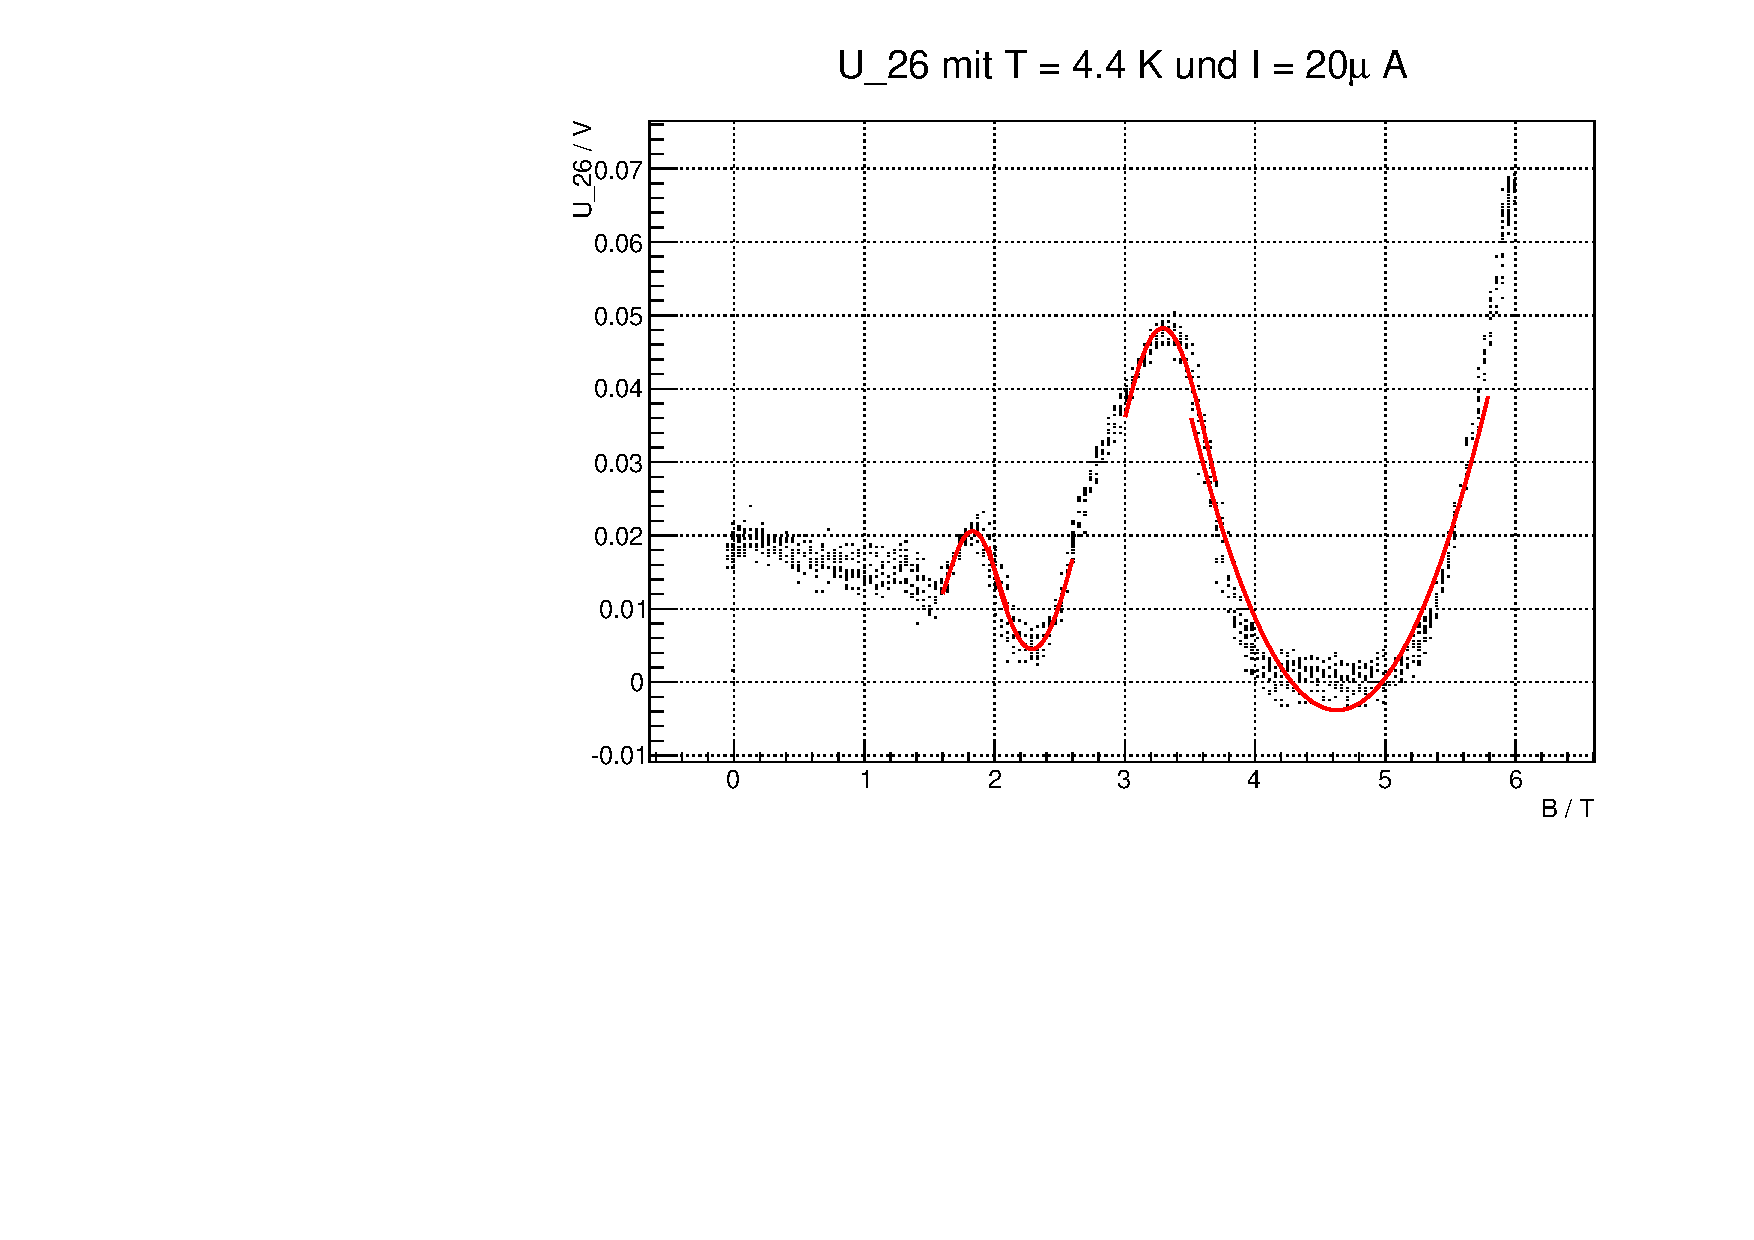
\includegraphics[scale = 0.5]{../plots/U_26_20muA_4400mK.pdf}
\caption{Längsspannung $\mathrm{U_{26}}$ für I=20 $\mathrm{\mu}$A und T=4.4 K.}
\end{figure}

\begin{figure}
\label{}
\centering
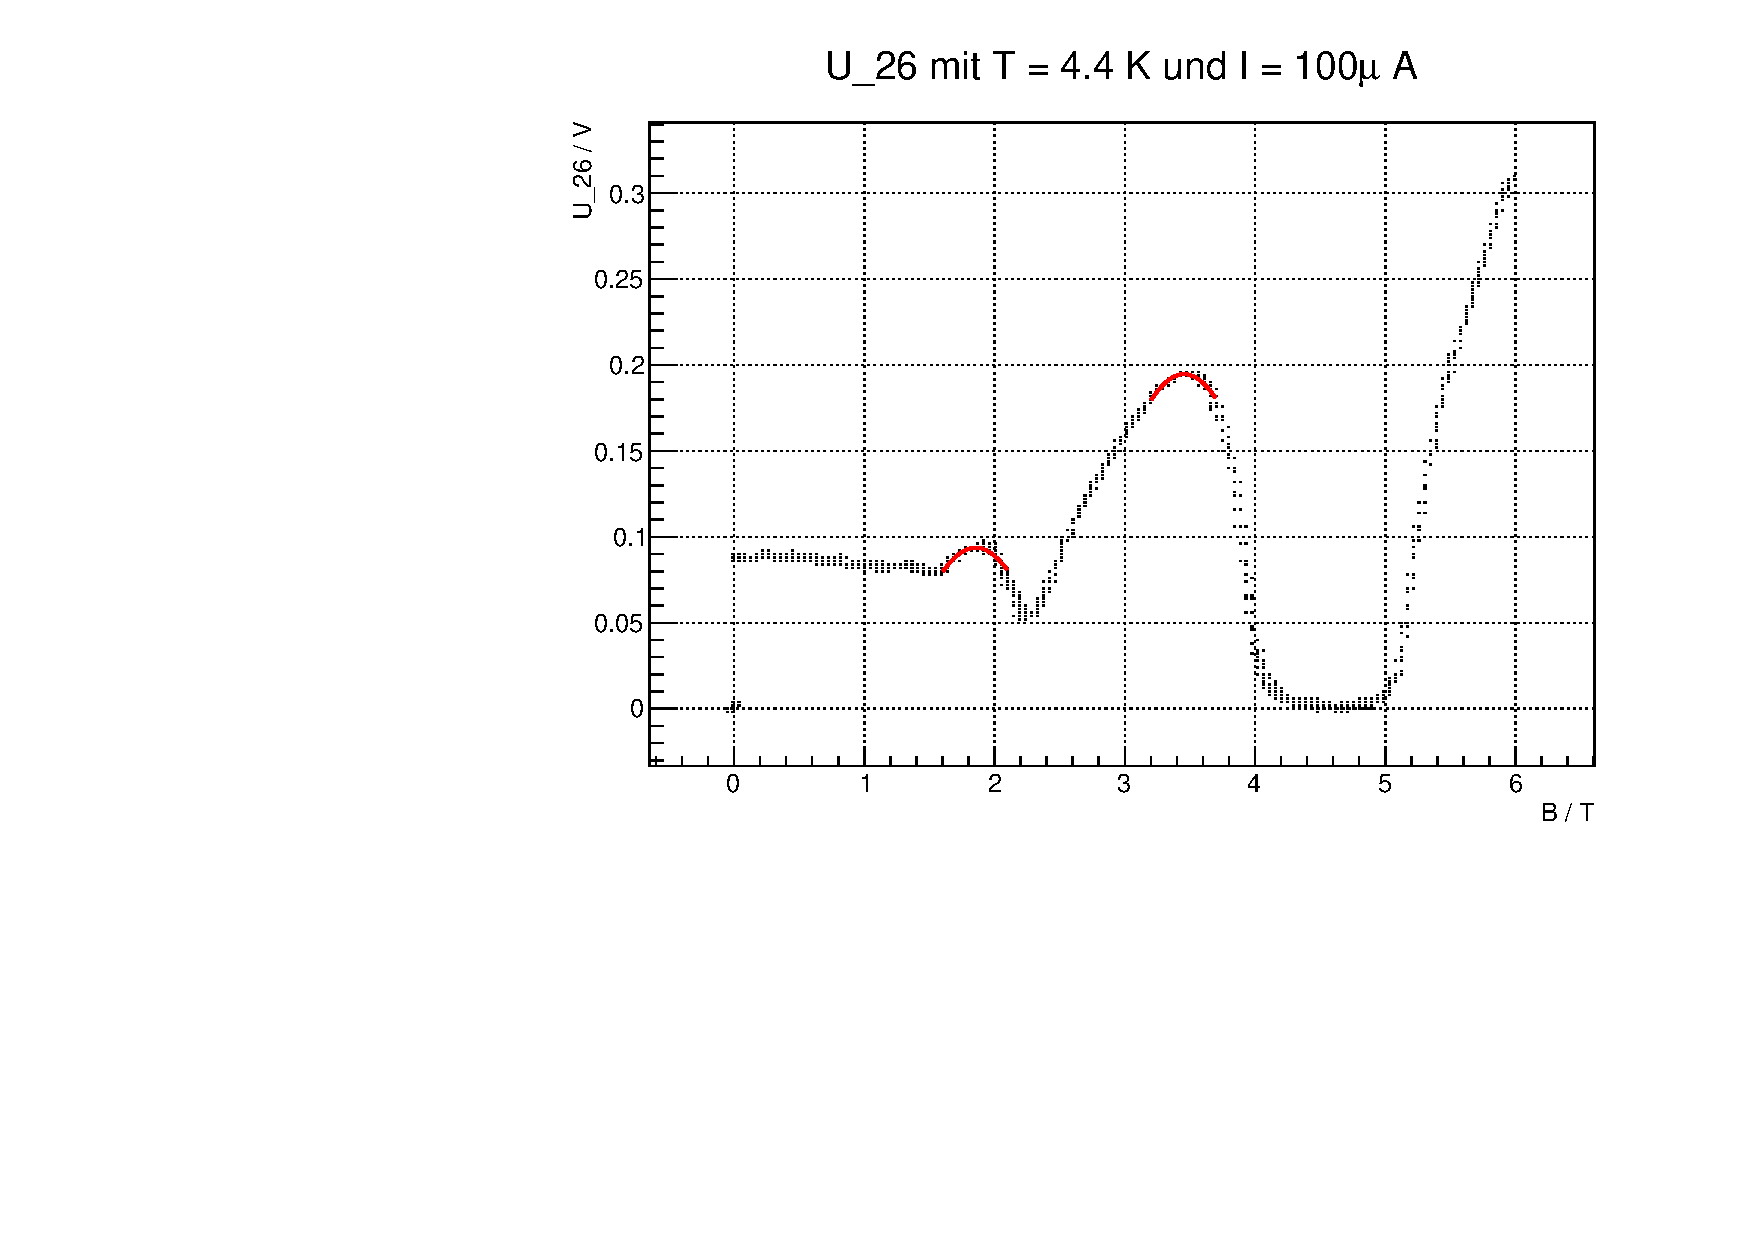
\includegraphics[scale = 0.5]{../plots/U_26_100muA_4400mK.pdf}
\caption{Längsspannung $\mathrm{U_{26}}$ für I=100 $\mathrm{\mu}$A und T=4.4 K.}
\end{figure}

\newpage

\begin{figure}
\label{}
\centering
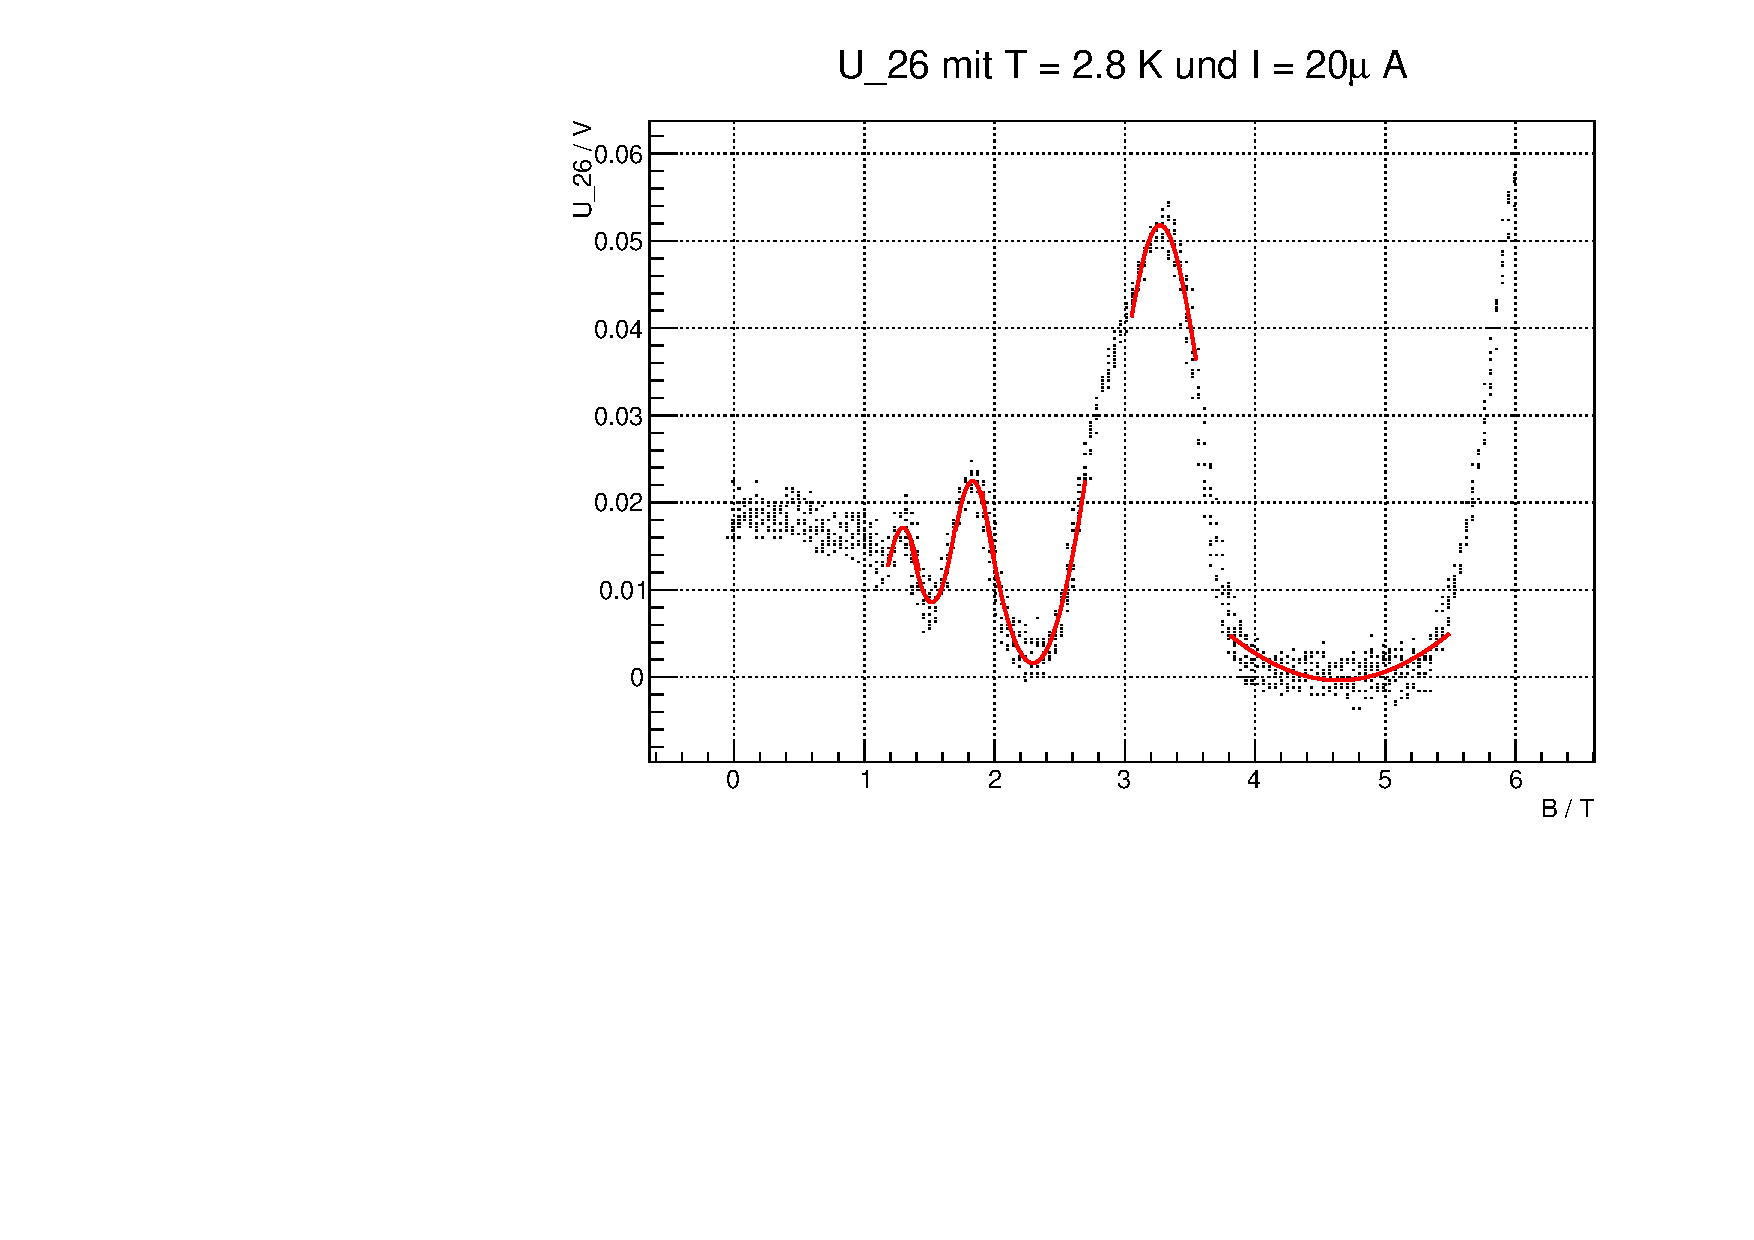
\includegraphics[scale = 0.5]{../plots/U_26_20muA_2800mK.pdf}
\caption{Längsspannung $\mathrm{U_{26}}$ für I=20 $\mathrm{\mu}$A und T=2.8 K. Die Daten für diesen Plot stammen von einer anderen Gruppe.}
\end{figure}

\begin{figure}
\label{}
\centering
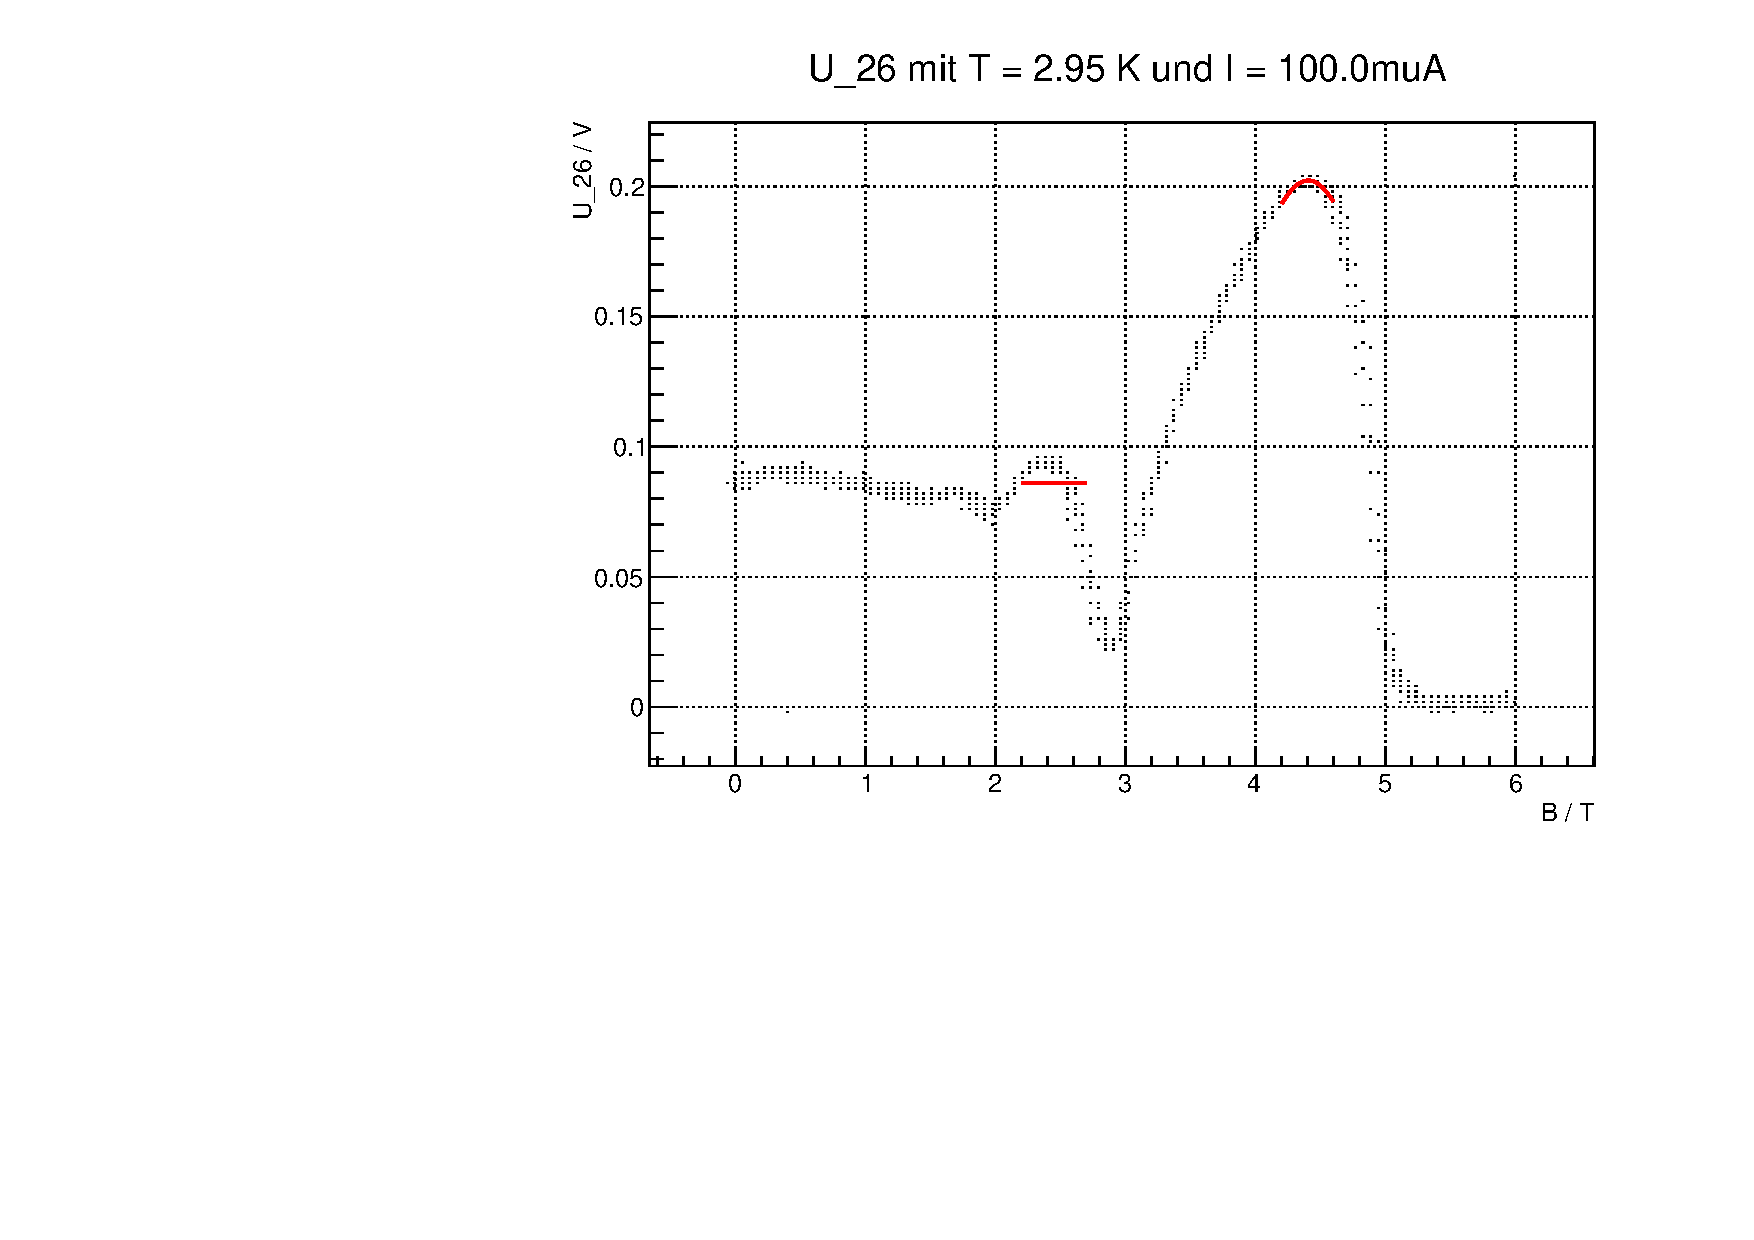
\includegraphics[scale = 0.5]{../plots/U_26_100muA_2950mK.pdf}
\caption{Längsspannung $\mathrm{U_{26}}$ für I=100 $\mathrm{\mu}$A und T=2.95 K. Die grüne senkrechte Linie gibt an, wann es zum Quenchen kam. Die Werte danach können nicht mehr verwendet werden, da das Magnetfeld herunter gefahren wurde. Aus rechnerischen Gründen wurde die Magnetfeldskala dennoch weitergeführt.}
\end{figure}

\newpage


\FloatBarrier

\subsubsection{Hall-Plateaus}
Wie in der Vorbereitung beschrieben, sind in der Hallspannung Plateaus zu sehen. Um diese genauer zu bestimmen, wurden horizontale Geraden in den jeweiligen Wertebereichen an die Spannungswerte gefittet. Dadurch wird der Spannungswert genauer bestimmt. Abb.7-10 zeigen die vier aufgenommenen Kurven, Abb.6 zeigt die Ergebnisse der Fits und die zugehörigen Bereiche des Magnetfeldes.


\subsubsection{Identifikation der Plateuas}
Es gilt die Gleichung\footnote{Bianca Müller: Staatsexamensarbeit: Der Quanten-Hall-Effekt im Fortgeschrittenenpraktikum, Physikalisches Institut der Universität Karlsruhe (TH), Dezember 1997}: 
$$\frac{U_H}{I} = \frac{h}{i \cdot e^{2}} $$
mit der Hallspannung $U_H$, dem angelegten Strom I und dem Füllfaktor i. In obiger Tabelle, Abb.6, ist dieser Füllfaktor für jedes Plateau mit angegeben. Dabei wurde die Bedingung ausgenutzt, dass i eine ganze Zahl sein muss; bei der Berechnung lag diese Zahl aber nie weiter als eine Standardabweichung von dem ungerundeten Wert entfernt.


\begin{figure}[h]
\centering
\caption{Spannungswerte und Magnetfeldstärken an den Maxima.}
\vspace*{0.5cm}
\begin{tabular}{ccccc}
\hline
Stromstärke in $\mathrm{\mu A}$ & Temperatur in $\mathrm{K}$ & B in $\mathrm{T}$ & $U_H$ in $\mathrm{V}$ & Füllfaktor i\\
\hline
\hline
20 & 2.73  & 1.4 ... 1.6 & $(8.418 \pm 0.026) \cdot 10^{-2}$ & 6\\
	&		& 2.3 ... 2.7 & $(1.369 \pm 0.002) \cdot 10^{-1}$ & 4	\\
	&		& 3.7 ... 5.5 & $(2.584 \pm 0.0008) \cdot 10^{-1}$ & 2 \\
20  & 4.1  & 2.0 ... 2.7 & $(1.315 \pm 0.003) \cdot 10^{-1}$ & 4\\
	&		& 4.0 ... 5.3 & $(2.636 \pm 0.002) \cdot 10^{-1}$ & 2\\
100	& 2.83	& 2.1 ... 2.3 & $(6.459 \pm 0.009) \cdot 10^{-1}$ & 4\\
	&		& 4.0 ... 5.3 & $1.306 \pm 0.0003$ & 2\\
100 & 4.4  & 2.2 ... 2.4 & $(6.565 \pm 0.012) \cdot 10^{-1}$ & 4\\
	&		& 4.0 ... 5.2 & $1.303 \pm 0.0003$ & 2 \\
\hline
\end{tabular}
\end{figure}

\FloatBarrier
\newpage

\begin{figure}
\label{}
\centering
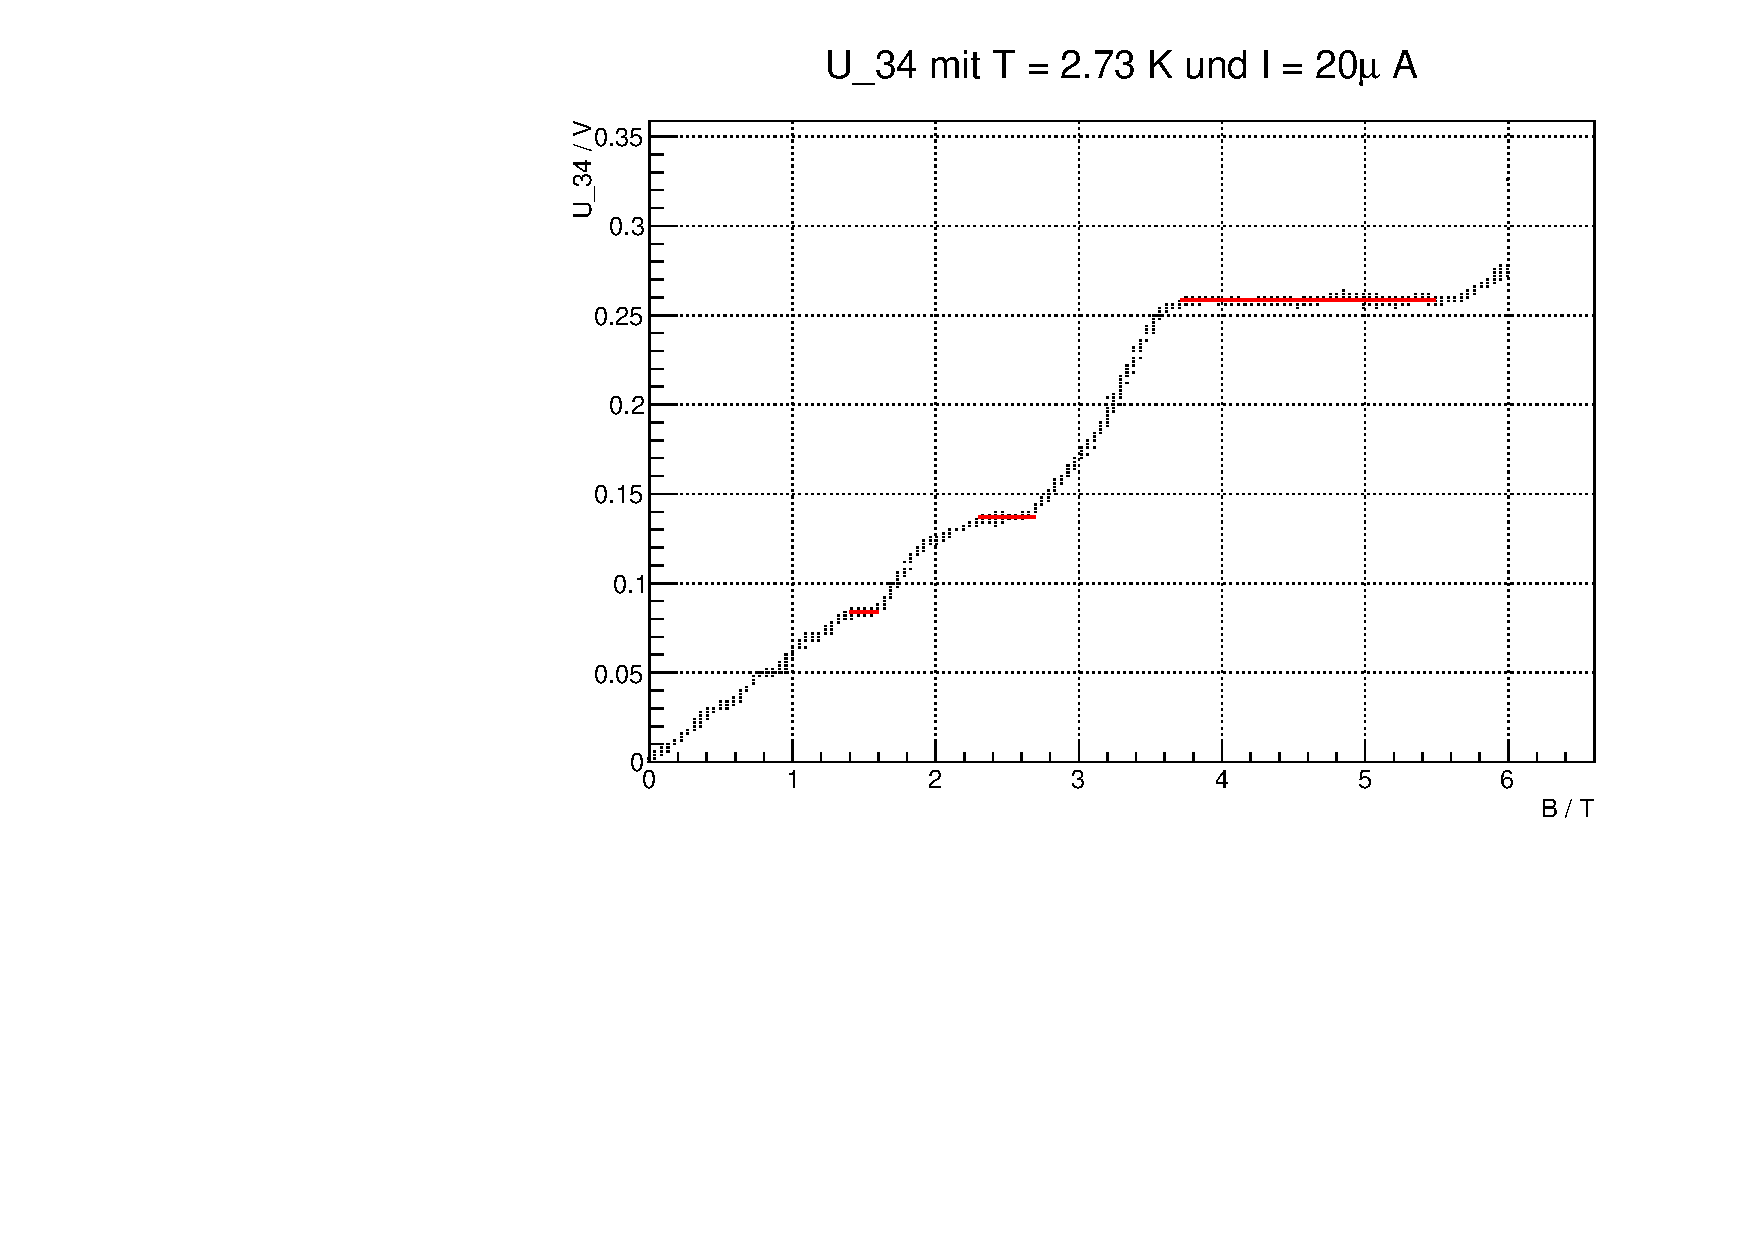
\includegraphics[scale = 0.5]{../plots/U_34_20muA_2730mK.pdf}
\caption{Hallspannung $\mathrm{U_{34}}$ für I=20 $\mathrm{\mu}$A und T=2.73 K}
\end{figure}

\begin{figure}
\label{}
\centering
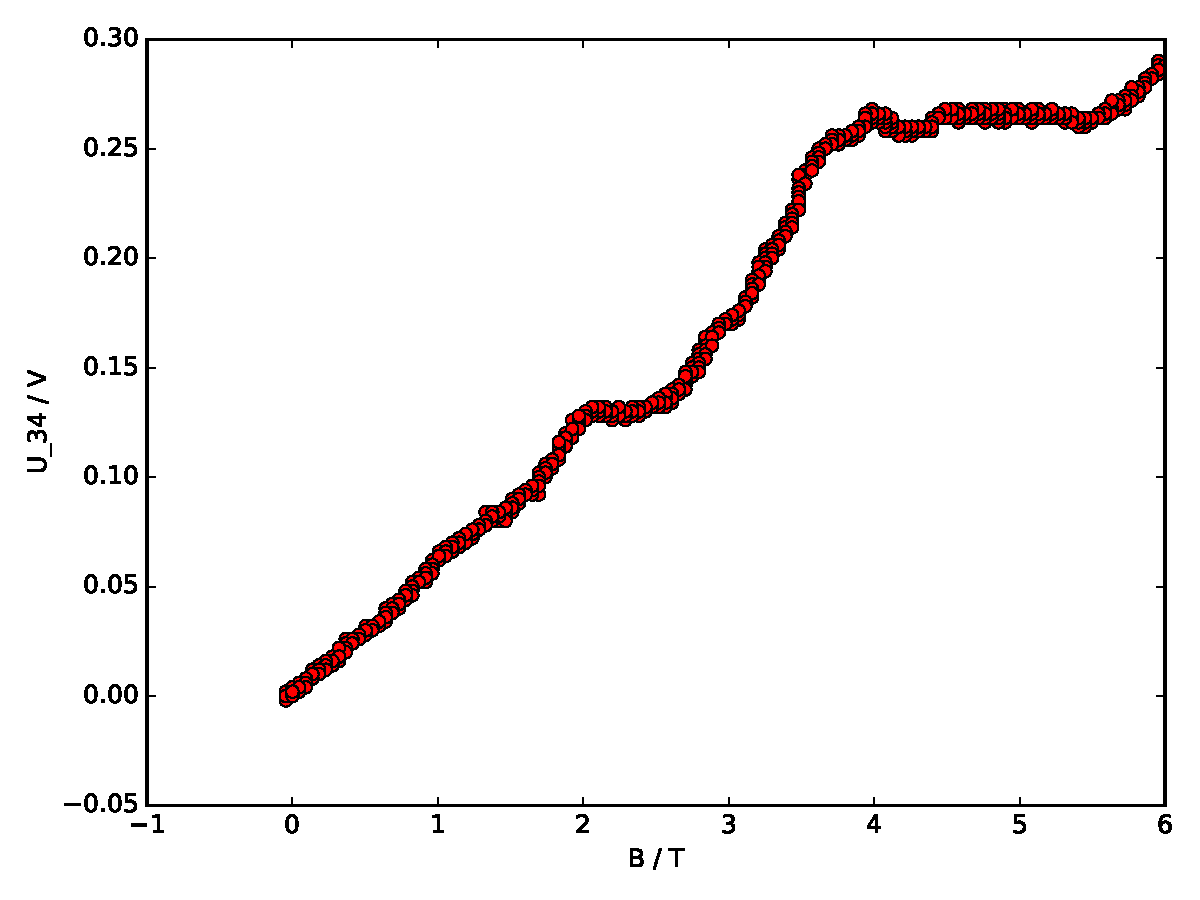
\includegraphics[scale = 0.5]{../plots/U_34_20muA_4100mK.pdf}
\caption{Hallspannung $\mathrm{U_{34}}$ für I=20 $\mathrm{\mu}$A und T=4.1 K}
\end{figure}

\newpage

\begin{figure}
\label{}
\centering
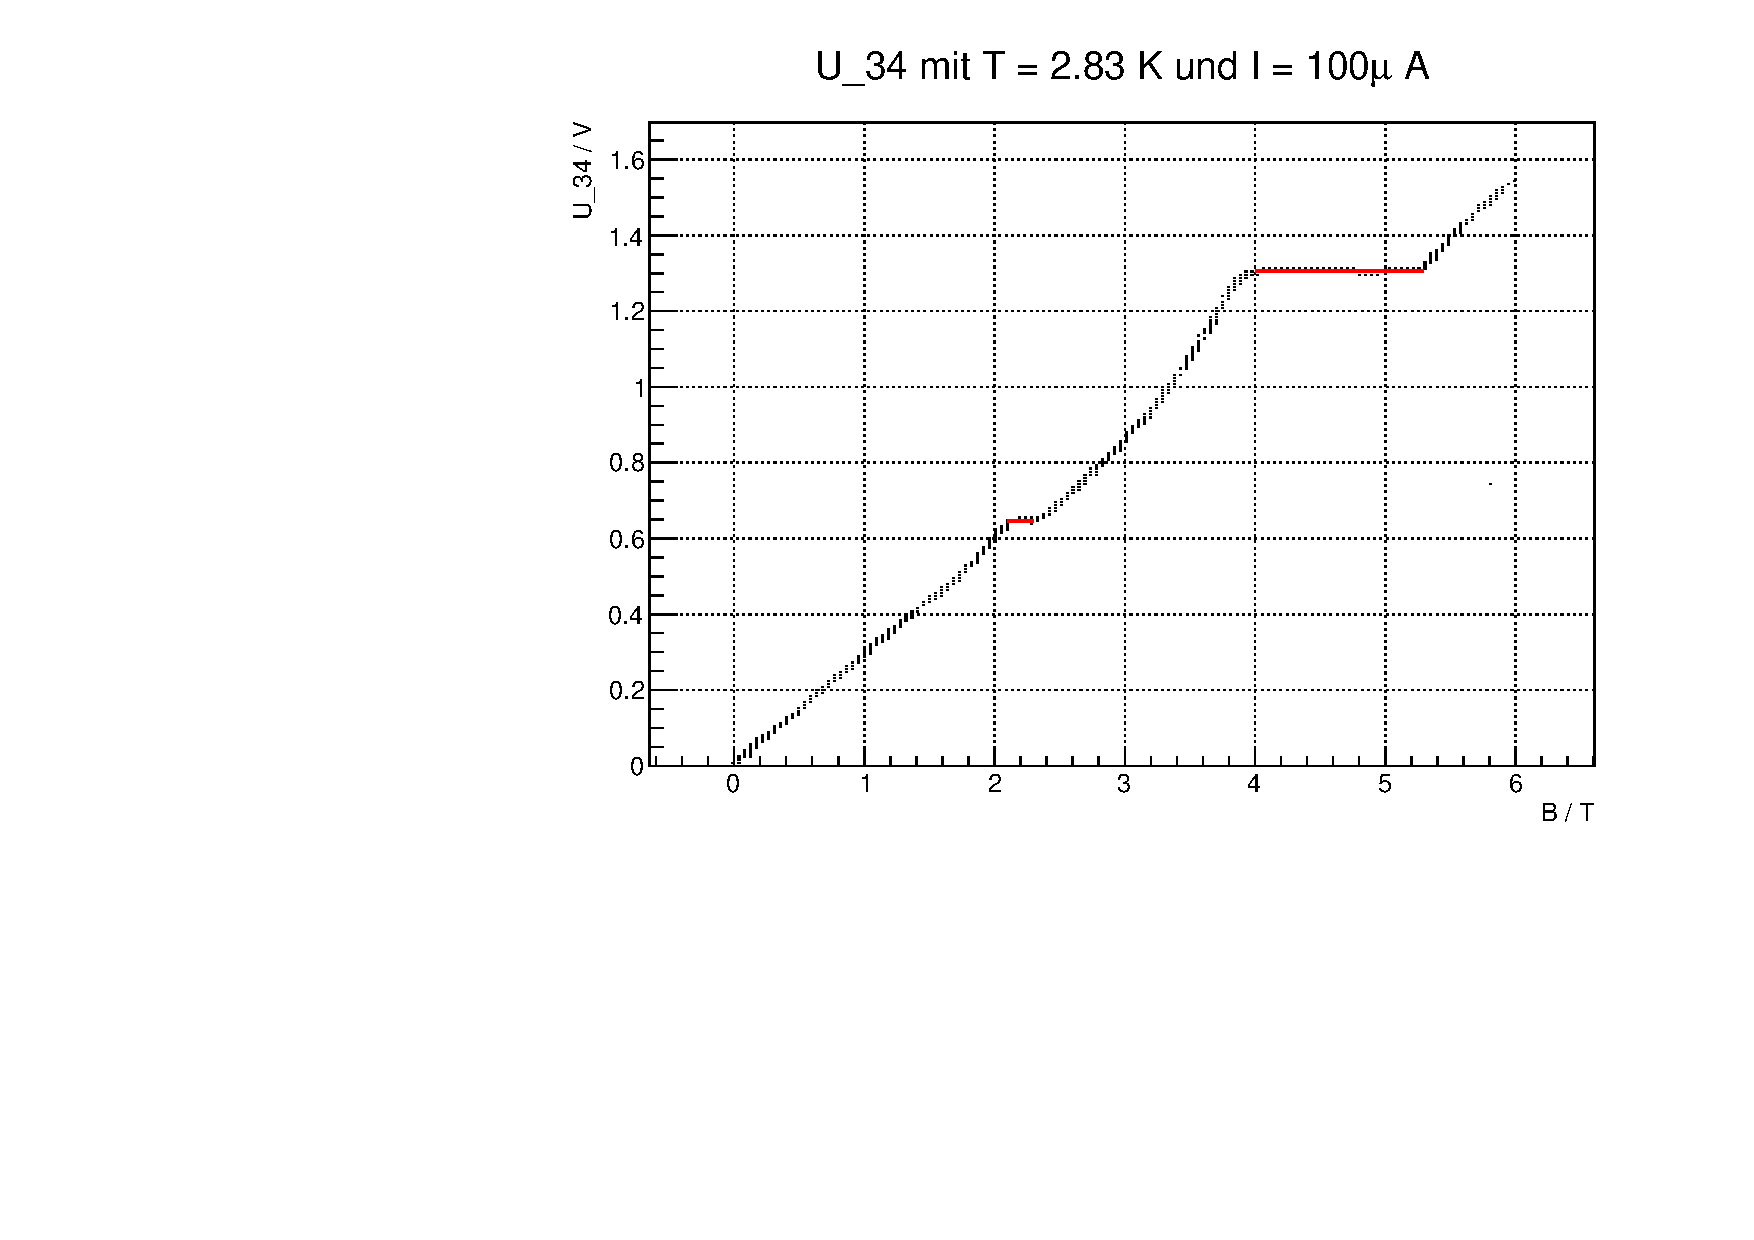
\includegraphics[scale = 0.5]{../plots/U_34_100muA_2830mK.pdf}
\caption{Hallspannung $\mathrm{U_{34}}$ für I = 100 $\mathrm{\mu}$A und T=2.83 K}
\end{figure}

\begin{figure}
\label{}
\centering
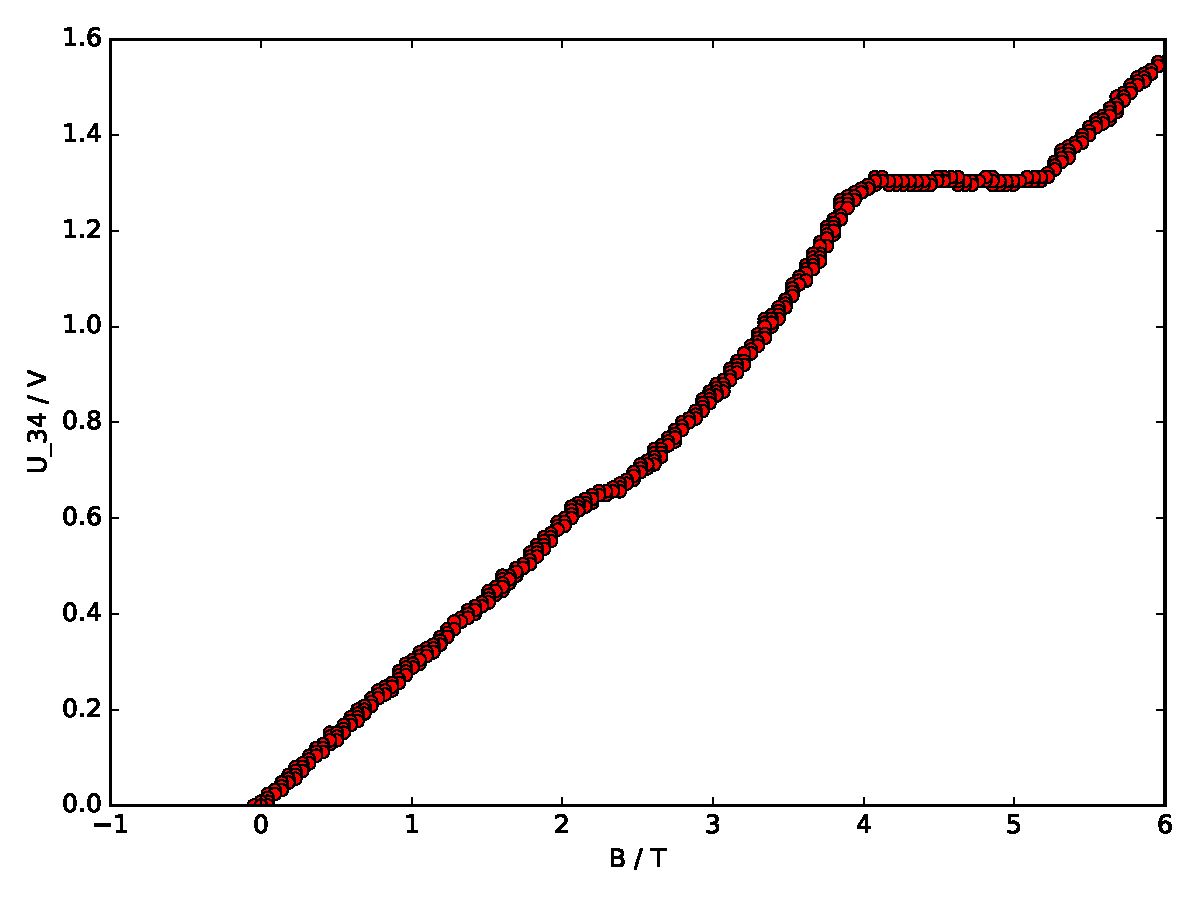
\includegraphics[scale = 0.5]{../plots/U_34_100muA_4400mK.pdf}
\caption{Hallspannung $\mathrm{U_{34}}$ für I=100 $\mathrm{\mu}$A und T=4.4 K}
\end{figure}

\FloatBarrier
\newpage


\subsubsection{Ladungsträgerkonzentration}
Die Flächenladungsträgerdichte $n_s$ eines 2DEG wird berechnet aus
$$n_s = \frac{B}{U_H \cdot e} \cdot I $$
Sie ist quantisiert und abhängig von dem jeweiligen Hall-Plateau. Zur Berechnung wird jeweils das Magnetfeld am Maximum in der Längsspannung genommen. Mit dem Entartungsgrad $N$ hängt sie über $n_s = i \cdot N$ zusammen. \\
Für $I = 20 \ \mathrm{\mu A}$ bei $T = 2.73 \ \mathrm{K}$ werden wie bereits erwähnt die Daten einer anderen Gruppe verwendet. In Abb.1 sind diese auch eingetragen. \\
In Abb.11 ist $n_s$ für jedes Plateau aufgelistet. Die Reihenfolge ist dieselbe wie in Abb.6. \\
\paragraph{Fehlerrechnung} Für die Fehlerrechnung wird die Gauß'sche Fehlerfortpflanzung verwendet. Da in obiger Gleichung $B$, $U_H$ systematische sowie statistische Unsicherheiten haben und $I$ eine systematische Unsicherheit hat, folgt für die jeweiligen Fehler
$$\sigma _{n_s, stat.}^{2} = (\frac{B}{U_H e} \cdot \sigma _{I, stat.})^{2} + (\frac{B \cdot I}{U_H^{2} e} \cdot \sigma _{U_H, stat.})^{2}$$
$$\sigma _{n_s, sys.}^{2} = (\frac{I}{U_H e} \cdot \sigma _{B, sys.})^{2} + (\frac{B}{U_H e} \cdot \sigma _{I, sys.})^{2} + (\frac{B \cdot I}{U_H^{2} e} \cdot \sigma _{U_H, sys.})^{2}$$
Die statistischen Unsicherheiten folgen aus den entsprechenden Funktionsanpassungen. Die systematischen werden wie folgt abgeschätzt: \\
Die Stromstärke kann durch das Messgerät in dem verwendeten Bereich recht gut eingestellt werden, wie in dem zugehörigen Datenblatt steht. Hierfür nehmen wir einen systematischen Fehler von $\sigma _{I, sys.} = 0.01 \ \mathrm{\mu A}$ an. Für $U_H$ und $B$ dient die Auflösung des jeweilige Messbereiches des Oszilloskops als Anhaltspunkt. Hier nehmen wir $\sigma _{U_H, sys.} = 0.004 \ \mathrm{V}$ und $\sigma _{B, sys.} = 0.004 \ \mathrm{T}$. \\
In unten stehender Tabelle sind beide Unsicherheiten mit eingetragen, wobei durchgehend zuerst der systematische, dann der statistische Fehler angegeben wird.

\begin{figure}
\centering
\caption{Flächenladungsträgerdichte $n_s$ für jedes Hall-Plateau mit Messunsicherheiten. Es wird immer zuerst der systematische, dann der statistische Fehler angegeben.}
\vspace*{0.5cm}
\begin{tabular}{ccccc}
\hline
$I$ in $\mathrm{\mu A}$ & $T$ in $\mathrm{K}$ & $B$ in $\mathrm{T}$ & $U_H$ in $\mathrm{V}$ & $n_s$ in $10^{11} \ \mathrm{cm^{-2}}$ \\
\hline
\hline
20 & 2.73  & $1.297 \pm 0.006$ & $(8.418 \pm 0.026) \cdot 10^{-2}$ & $1.923 \pm 0.092 \pm 0.011$\\
	&		& $1.830 \pm 0.005$ & $(1.369 \pm 0.002) \cdot 10^{-1}$ & $1.669 \pm 0.049 \pm 0.005$	\\
	&		& $3.272 \pm 0.004$ & $(2.584 \pm 0.0008) \cdot 10^{-1}$ & $1.581 \pm 0.025 \pm 0.002$ \\
20  & 4.1  & $1.831 \pm 0.004$ & $(1.315 \pm 0.003) \cdot 10^{-1}$ & $1.738 \pm 0.053 \pm 0.005$\\
	&		& $3.292 \pm 0.004$ & $(2.636 \pm 0.002) \cdot 10^{-1}$ & $1.559 \pm 0.024 \pm 0.002$\\
100	& 2.83	& $2.369 \pm 0.007$ & $(6.459 \pm 0.009) \cdot 10^{-1}$ & $2.289 \pm 0.015 \pm 0.007$\\
	&		& $4.406 \pm 0.006$ & $1.306 \pm 0.0003$ & $2.106 \pm 0.007 \pm 0.003$\\
100 & 4.4  & $1.855 \pm 0.004$ & $(6.565 \pm 0.012) \cdot 10^{-1}$ & $1.764 \pm 0.011 \pm 0.005$\\
	&		& $3.455 \pm 0.003$ & $1.303 \pm 0.0003$ & $1.655 \pm 0.005 \pm 0.001$ \\
\hline

\end{tabular}

\end{figure}

\newpage

\subsection{Feinstrukturkonstante}
Die Feinstrukturkonstante wird wie in der Vorbereitung erwähnt berechnet durch folgende Gleichung:
$$\frac{U_H}{I} = \alpha ^{-1} \cdot \mu _0 c / (2 \cdot i) $$
Für die magnetische Feldkonstante und die Lichtgeschwindigkeit werden die Werte aus der Vorbereitungsmappe Anhang 4 \footnote{Tabelle der empfohlenen konsistenten Werte der Naturkonstanten (CODATA 1986)} verwendet:
$$\mu _0 = 4 \pi \cdot 10^{7} \ \mathrm{\frac{N}{A^{2}}} $$
$$c = 299792458 \ \mathrm{\frac{m}{s}} $$
Damit wird $\alpha$ berechnet. Der Füllfaktor $i$ wird der Tabelle in Abb.6 entnommen.\\
\paragraph{Fehlerrechnung}
Die Hallspannung $U_H$ hat sowohl eine statistische, als auch eine systematische Unsicherheit. Als weitere fehlerbehaftete Größe gibt es noch die Stromstärke mit einem systematischen Fehler. Die Gauß'sche Fehlerfortpflanzung liefert in diesem Fall:
$$\sigma _{\alpha, sys.}^{2} = (\frac{\mu _0 c}{2 \cdot i})^{2} \cdot ((\frac{\sigma _{I, sys.}}{U_H})^{2} + (\frac{I \cdot \sigma _{U_H, sys.}}{U_H ^{2}})^{2}) $$
$$\sigma _{\alpha, stat.}^{2} = (\frac{\mu _0 c}{2 \cdot i})^{2} \cdot (\frac{I \cdot \sigma _{U_H, stat.}}{U_H ^{2}})^{2} $$
Zur Bestimmung der systematischen Messunsicherheit wird wie bei der Bestimmung der Flächenladungsträgerdichte diskutiert $\sigma _{U_H, sys.} = 0.004 \ \mathrm{V}$ und $\sigma _{I, sys.} = 0.01 \ \mathrm{\mu A}$ abgeschätzt. \\
Die statistische Unsicherheit folgt aus den oben durchgeführten Fits. Zusätzlich werden die für die jeweiligen Füllfaktoren berechneten Werte in einen Graphen aufgetragen und mit einer horizontalen Ausgleichsgeraden gefittet. Das ergibt die endgültige statistische Unsicherheit, die systematische ist davon unabhängig und muss quadratisch addiert werden. Das ist in Abb.12 zu sehen. Es wurde noch  der Literaturwert nach Anhang 4 der Literaturmappe\footnote{Tabelle der empfohlenen konsistenten Werte der Naturkonstanten (CODATA 1986)} von $\alpha _{theo} = \frac{1}{137.0359895} = 7.29735308 \cdot 10^{-3}$ eingezeichnet.\\
Die Feinstrukturkonstante haben wir somit bestimmt zu:
$$\alpha = (7.228 \pm 0.493 \ (sys.) \pm 0.001 \ (stat.)) \cdot 10^{-3}$$


\begin{figure}[h]
\centering
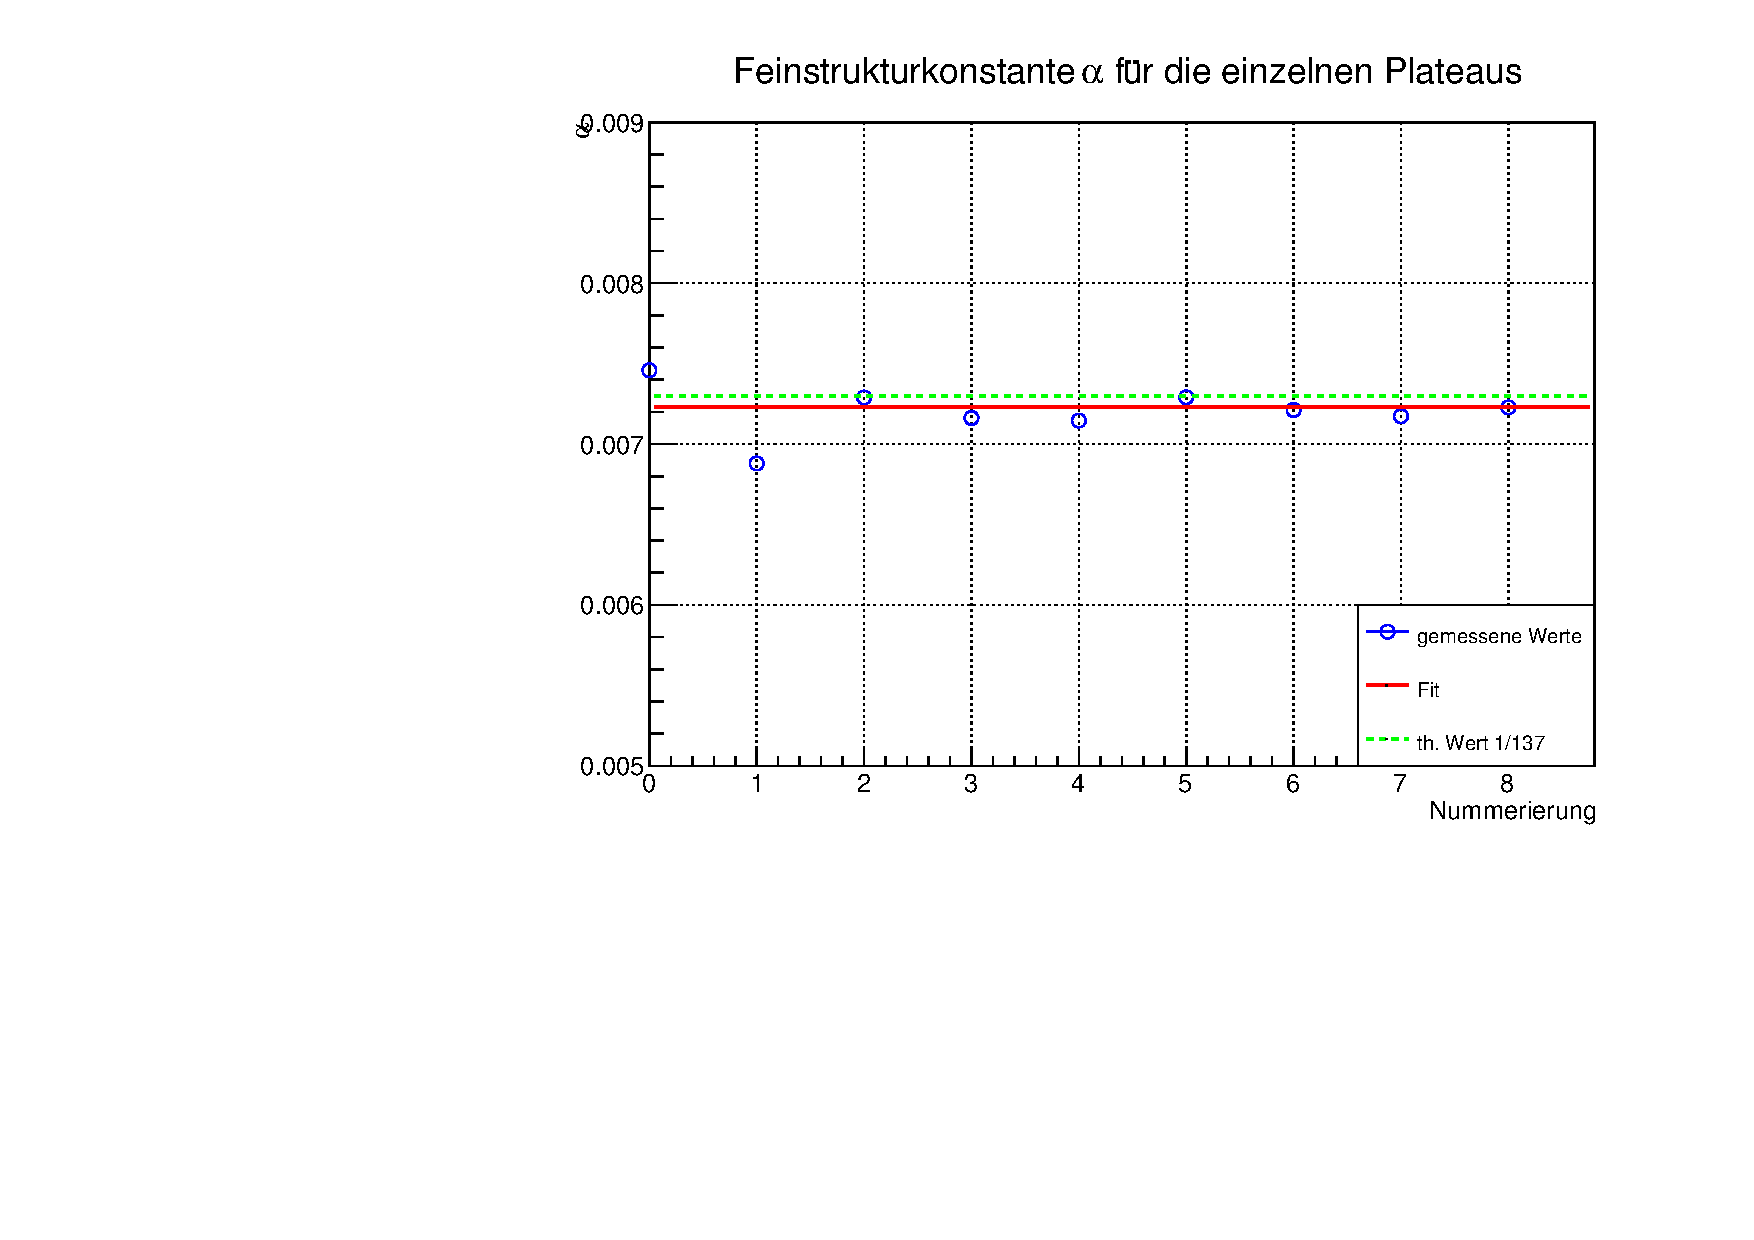
\includegraphics[scale=0.45]{../plots/alpha.pdf}
\caption{Feinstrukturkonstante $\alpha$ für jedes Plateau und horizontaler Fit. Gestrichelt ist der im Text erwähnte Literaturwert eingezeichnet. Die Nummerierung ist analog zu Abb.6. Oberster Eintrag in der Tabelle entspricht dem Wert mit der kleinsten Nummerierung.}
\end{figure}


\subsection{Literaturvergleich}
Der oben angegebene Literaturwert der Feinstrukturkonstanten liegt innerhalb einer Standardabweichung von unserem Ergebnis. Von daher ist das Ergebnis zufriedenstellend. Allerdings ist der systematische Fehler sehr groß im Vergleich zum statistischen. Das lässt vermuten, dass er eventuell etwas zu groß abgeschätzt wurde. Eine genauere Kenntnis der verwendeten Messapparaturen und tiefgehendere Untersuchungen könnten zu einer besseren Abschätzung führen.